\begin{document}

\subsection{Что такое Box model? Раскройте суть Box model.}

Box model -- это синтетическая модель для ознакомления с базовыми возможностями гидродинамического симулятора.

Box model представляет собой параллелепипед с блочно-центрированной сеткой.

У всех ячеек Box модели одинаковые пористости и проницаемости.

В модели заданы ОФП и PVT-свойства.

Скважины в Box модели размещены по 5-точечной схеме.
\\

\textbf{Описание входного .data файла Box модели.}

\underline{Секция RUNSPEC}

Секция \textbf{RUNSPEC} необходима симулятору для выделения оперативной памяти для хранения данных (значений параметров) модели.
Точное количество памяти требует Eclipse.
В т-Навигаторе память выделяется динамически, поэтому в т-Навигаторе некоторые данные этого раздела игнорируются. 

Зададим название модели, присутствующие в ней фазы (нефть и вода) и метрическую систему единиц.

\begin{eclrun}
NOECHO
RUNSPEC

TITLE
Test_model

OIL
WATER

METRIC
\end{eclrun}

Если хотим только прочитать файл и проверить его на наличие ошибок без запуска расчёта, то используем ключевое слово NOSIM.
Но в данной модели хотим запустить полный расчёт, поэтому закомментируем это ключевое слово.
\begin{eclrun}
-- NOSIM
\end{eclrun}

Зададим количество $Nx$, $Ny$ и $Nz$ ячеек расчётной сетки в направлениях $X$, $Y$, $Z$.

\begin{eclrun}
DIMENS
-- Nx  Ny   Nz
   61  114  40 /
\end{eclrun}

Следующее ключевое слово используется для определения числа областей с различными параметрами моделирования.
Задаваемые числа определяют количество областей с различными свойствами начального равновесия.
В данном примере определим только число регионов (равное 1) с различными начальными данными опции равновесия (эти данные будут задаваться в дальнейшем с помощью ключевого слова EQUIL).
\begin{eclrun}
EQLDIMS
 1  /
\end{eclrun}

Следующее ключевое слово задаёт максимальное число параметров, описывающих аквифер.
Первые 4 по умолчанию; максимальное число водоносных пластов, описанных с помощью аналитической модели, в рассматриваемом примере равно 1; максимальное число блоков сетки, примыкающих к какому-либо водоносному пласту, равно 100000; следующие 2 параметра по умолчанию. Подробнее в руководстве.
\begin{eclrun}
AQUDIMS
  4*  1  100000 /
\end{eclrun}

Укажем, что в модели будет использоваться метод масштабирования конечных точек фазовых проницаемостей и капиллярных давлений.
В параметрах указываются переключатель направленного масштабирования конечных точек (в данном примере NODIR) и переключатель нереверсивного масштабирования конечных точек (в данном примере REVERS).
\begin{eclrun}
ENDSCALE
'NODIR'  'REVERS' /
\end{eclrun}

Следующее ключевое слово задаёт максимальные размерности данных по скважинам.
Всего 12 параметров.
В данном примере зададим только максимальное количество скважин в модели, максимальное количество интервалов перфорации для каждой скважины, максимальное количество групп скважин в модели, максимальное количество скважин в одной группе; остальные параметры оставим по умолчанию равными нулю. 
\begin{eclrun}
WELLDIMS
-- Max_wells  Conn_well  Max_groups  Wells_group
   30         50         2           30   /
\end{eclrun}

Следующее ключевое слово используется для задания числа регионов с различными параметрами моделирования.
В данном примере зададим количество регионов фильтрации, количество регионов с различными PVT-свойствами, макимальное количество различных насыщенностей, задаваемых в одной VPT таблице, максимальное количество различных давлений, задаваемых в одной VPT таблице, количество регионов, для которых необходимо выводить данные о запасах; остальные параметры оставим по умолчанию.
\begin{eclrun}
TABDIMS
--NTSFUN  NTPVT  NSSFUN_nodes  NPPVT_nodes NTFIP
    1      1       30           20         3 /
\end{eclrun}

Следующее ключевое слово используется для задания числа регионов с различными параметрами моделирования.
Задаваемые 4 числа определяют:
количество регионов, для которых необходимо выводить данные о запасах (может быть задано также с помощью TABDIMS);
количество множеств регионов, для которых необходимо выводить данные о запасах;
количество регионов с независимыми месторождениями;
количество регионов потока.

В данном примере зададим только первый параметр (который фактически уже задали в TABDIMS); значения остальных параметров оставим по умолчанию.
\begin{eclrun}
REGDIMS
--fipnum fipxx isolnum fluxnum 
 3  /
\end{eclrun}

Укажем максимальное количество векторов в summary файле.
\begin{eclrun}
SMRYDIMS
1000000  /
\end{eclrun}

Выходные и входные файлы унифицированы.
\begin{eclrun}
UNIFOUT
UNIFIN
\end{eclrun}

Укажем дату начала моделирования.
\begin{eclrun}
START
1 'NOV' 2022 /
\end{eclrun}

Включим возможность использования опций обработки данных сетки
\begin{eclrun}
GRIDOPTS
YES /
\end{eclrun}

Зададим ограничения на печать сообщений разных типов, а также условия на остановку расчёта при большом количестве сообщений.
\begin{eclrun}
MESSAGES
-- print                                            
-- message comment warning problem  error   bug     
   1000000 1000000 1000000 10000000 1000000 1000000
-- stop
-- message comment warning problem error bug
   1000000 1000000 1000000 100000  1000  1000  /
\end{eclrun}

\underline{Секция GRID}

Секция \textbf{GRID} необходима для задания геометрии и фильтрационно-ёмкостных свойств (ФЕС) модели.

Ключевое слово EQUALS позволяет задать значение любого параметра сетки для ячеек, выбранных в область параллелепипеда.

Зададим размеры ячеек DX, DY, DZ в направлениях X, Y, Z соответственно. По умолчанию размеры задаются для каждой из ячеек сетки. 
При этом симулятор строит блочно-центрированную геометрию сетки.
В дальнейшем (уже за рамками данного примера) будем использовать и геометрию угловой точки (с помощью ключевых слов COORD и ZCORN).
\begin{eclrun}
GRID

EQUALS
'DX'    100  /
'DY'    100  /
'DZ'    0.2  /
/
\end{eclrun}


Далее зададим глубину залегания верхнего слоя ячеек.
После значения 2000 заданы 4 параметра по умолчанию (начало интервала по X, конец интервала по X, начало интервала по Y, конец интервала по Y -- по умолчанию заданы все ячейки в направлениях X и Y) и два параметра (начало интервала по Z, конец интервала по Z) равны 1 (т.е. задаём ячейки только верхнего слоя).
Таким образом, значение TOPS 2000 применяется только к ячейкам верхнего слоя. Для других слоёв симулятор автоматически определяет значение, основываясь на высоте ячеек. 
\begin{eclrun}
EQUALS
'TOPS' 2000 4* 1 1 /
/
\end{eclrun}

Далее определяем, что все ячейки модели активны, и задаём пористость и проницаемость по X, Y, Z во всех ячейках.
\begin{eclrun}
EQUALS
'ACTNUM'  1  /
'PORO'  0.2  /
'PERMX' 100  /
'PERMY' 100  /
'PERMZ'  1  /
/
\end{eclrun}

Скажем симулятору, что необходимо записать исходные данные со свойствами сетки и таблицами насыщенностей в файл, который в дальнейшем можно будет прочесть в графических пакетах.
\begin{eclrun}
INIT
\end{eclrun}

\underline{Секция EDIT}

Опциональная секция с возможностью редактирования данных \textbf{GRID} секции.
В данном примере оставим эту секцию пустой.
\begin{eclrun}
EDIT
\end{eclrun}

\underline{Секция PROPS}

Секция \textbf{PROPS} необходима для задания параметров флюидов, относительных фазовых проницаемостей и распределения жидкостей на основе функций капиллярных давлений.

Определим PVT-свойства воды.
Задаются опорное давление, коэффициент объёмного расширения воды, коэффициент сжимаемости воды, вязкость воды и производная вязкости воды по давлению.
\begin{eclrun}
PROPS

PVTW          
--P    Bw      cw        muw     dmuw/dpres  
159.6  1.0264  4.32E-05  0.3253  0  /
\end{eclrun}

Определим упругие свойства породы.
Задаются опорное давление, сжимаемость породы, сжимаемость скелета породы, сжимаемость блока (блока, содержащего смесь), значение пористости при опорном давлении, значение коэффициента Пуассона при опорном давлении.
В данном примере укажем значения только для опорного давления и сжимаемости породы; остальные параметры оставим по умолчанию (см. руководство).
\begin{eclrun}
ROCK
--Pref  Compr 
159.6  4.765E-05  /
\end{eclrun}

Зададим плотности нефти и воды в поверхностных условиях.
\begin{eclrun}
DENSITY 
860  1007.5  /
\end{eclrun}

Следующее ключевое слово служит для задания постоянной и однородной концентрации растворённого газа в нефти.
Это обеспечивает наиболее эффективное моделирование системы чёрная нефть, где нет отдельной газовой фазы и давление никогда не опускается ниже точки давления насыщения.

Указаны концентрация растворённого газа и давление насыщения (расчёт будет завершён, если давление в каком-либо блоке сетки опустится ниже этого значения).
\begin{eclrun}
RSCONST 
--Rs  Pb
  20  34  /
\end{eclrun}


Следующее ключевое слово используется для задания PVT-свойств нелетучей нефти для рассматриваемых PVT-регионов.

Необходимо ввести следующие параметры: давление насыщения, коэффициент объёмного расширения нефти, вязкость нефти при давлении насыщения.

PVT свойства нелетучей нефти для каждого PVT региона вводятся в таблицы.
Количество таблиц равно количеству регионов, определённых в TABDIMS.

В рассматриваемом примере одна таблица для единственного региона.
Таблица получена в Excel-файле при выполнении задания от 21.09.2022.

\begin{eclrun}
PVDO 
--P     Bo      muo
34     1.06000  9.00000
40     1.05926  9.08157
60     1.05681  9.35346
80     1.05436  9.62535
100    1.05192  9.89724
120    1.04948  10.16913
140    1.04705  10.44102
159.6  1.04467  10.70748
180    1.04220  10.98481
200    1.03978  11.25670
220    1.03737  11.52859
240    1.03497  11.80048
260    1.03257  12.07237
280    1.03018  12.34427
300    1.02779  12.61616
/
\end{eclrun}

Следующее ключевое слово можно указывать, если в секции \textbf{RUNSPEC} присутствует ключевое слово ENDSCALE.
Позволяет задать трёхточечный метод масштабирования конечных точек фазовых проницаемостей.
Указывается один аргумент, имеющий 2 возможных значения (YES -- да, трёхточечный метод масштабирования, NO -- нет, 2-точечный метод)
\begin{eclrun}
SCALECRS
YES /
\end{eclrun}


Зададим таблицы нормализованных относительных фазовых проницаемостей для систем вода-нефть для каждого региона фильтрации (количество регионов задано в TABDIMS -- в рассматриваемом примере один единственный регион -- следовательно, только одна таблица).

Таблица содержит 4 колонки со следующими параметрами: водонасыщенность (SW), проницаемость воды (KRWO), проницаемость нефти (KROW), капиллярное давление фазы нефть-вода (POW).
\begin{eclrun}
SWOF
--Sw     Krw     Kro     Pc
0.0  0.000000  1.000000  0.22100
0.1  0.049403  0.675833  0.11707
0.2  0.122172  0.436130  0.04704
0.3  0.207486  0.265435  0.02680
0.4  0.302128  0.149624  0.01752
0.5  0.404371  0.075953  0.01231
0.6  0.513110  0.033125  0.00900
0.7  0.627566  0.011364  0.00673
0.8  0.747156  0.002516  0.00507
0.9  0.871424  0.000191  0.00333
1.0  1.000000  0.000000  0.00000
/
\end{eclrun}

С помощью следующего ключевого слова задаём арифметические и алгебраические операции над параметрами сетки для ячеек, выбранных в область параллелепипеда.
Задаваемые значения: изменяемый параметр сетки; изменяемая область параллелепипеда; операция; параметр сетки, являющийся аргументом; скалярный параметр 1, если нужен; скалярный параметр 2, если нужен.

В рассматриваемом примере задаём корреляции остаточных насыщенностей и концевых точек от ФЕС ячейки.
Коэффициенты корреляций (скалярные параметры) найдены при выполнении задания от 21.09.2022.

Остаточные насыщенности и концевые точки необходимы для проведения масштабирования ранее заданных нормализованных ОФП.
\begin{eclrun}
OPERATE
SWCR   1 61  1 114  1 40  'LOGE'   PERMX /
SWCR   1 61  1 114  1 40  'MULTA'  SWCR  -0.04705  0.52721  /
SOWCR  1 61  1 114  1 40  'LOGE'   PERMX /
SOWCR  1 61  1 114  1 40  'MULTA'  SOWCR  -0.01289  0.27396 /
KRWR   1 61  1 114  1 40  'LOGE'   PERMX /
KRWR   1 61  1 114  1 40  'MULTA'  KRWR   0.06701  -0.14287 /
--Krw@(Sw=1-Sowcr)
/
\end{eclrun}

Далее для всех ячеек задаём:
максимальную водонасыщенность;
относительная проницаемость по нефти при критической водонасыщенности;
максимальное значение относительной проницаемости по нефти;
максимальное значение относительной проницаемости по воде
(все задаваемые значения используются при масштабировании конечных точек насыщенностей).
\begin{eclrun}
EQUALS
SWU 1 /--MAX Sw
KRORW  0.833 /--Kro@(Sw=Swcr)
KRO 1 /-- Kro@(SW=0)
KRW 1 /-- Krw@(SW=1)
/
\end{eclrun}

Далее зададим минимальную водонасыщенность ячеек SWL, используемую при масштабировании конечных точек насыщенностей (скопируем значения из критических водонасыщенностей SWCR).
\begin{eclrun}
COPY
SWCR SWL /--MIN Sw
/
\end{eclrun}


\underline{Секция REGION}

Секция \textbf{REGION} позволяет определить регионы (области) модели с разными свойствами.
В данном примере оставим эту секцию пустой.
\begin{eclrun}
REGIONS
\end{eclrun}


\underline{Секция SOLUTION}

В секции \textbf{SOLUTION} доопределяются параметры, необходимые для инициализации модели.

Следующее ключевое слово задаёт для каждого региона равновесия (в рассматриваемом примере один единственный регион) свойства, используемые при расчёте начальных условий.
Рассматривается равновесный способ инициализации.

Указаны: глубина; давление на этой глубине; глубина водо-нефтяного контакта; капиллярное давление на глубине водо-нефтяного контакта (если 0, то это зеркало свободной воды); глубина газо-нефтяного контакта; капиллярное давление на глубине газо-нефтяного контакта; далее см. руководство.

\begin{eclrun}
SOLUTION

EQUIL
--FWLs
2008   200.8   2008   0   1000   0  1  0  1*  /
\end{eclrun}

Следующее ключевое слово осуществляет управление выходными данными секции \textbf{SOLUTION}.
\begin{eclrun}
RPTSOL
'FIP=2' 'SWATINIT' /
\end{eclrun}

\underline{Секция SUMMARY}

В секции \textbf{SUMMARY} определяются векторы, которые запишутся в файлы с результатом расчёта, и их формат.

\begin{eclrun}
SUMMARY

ALL
SEPARATE
EXCEL
RUNSUM
RPTONLY
\end{eclrun}

\underline{Секция SCHEDULE}

В секции \textbf{SCHEDULE} определяются скважины, группы скважин, график работы, требования к отчётности и т.п.

Следующее ключевое слово осуществляет контроль вывода данных в restart файл.
\begin{eclrun}
SCHEDULE

RPTRST
--report every timestep
'BASIC=2' 'FREQ=1'  /
\end{eclrun}


Зададим структуру иерархии групп скважин.
\begin{eclrun}
GRUPTREE
'INJECT'  'FIELD'  /
'PRODUCE' 'FIELD'  /
/
\end{eclrun}

Следующее ключевое слово определяет информацию о забое скважин.

Вводятся следующие данные для каждой из скважин:
название скважины;
название группы скважин, к которой принадлежит данная скважина;
координата ячейки по оси X, в которой расположен забой или устье скважины;
координата ячейки по оси Y, в которой расположен забой или устье скважины;
опорная глубина для забойного давления (по умолчанию глубина первого интервала перфорации);
предпочтительная фаза для скважины (данные этого параметра используются для определения индекса продуктивности/приёмистости скважины, или её потенциального расхода);
далее см. руководство.

\begin{eclrun}
WELSPECS
-- name   group      iw  jw ref.depth phase
'INJ1'    'INJECT'   30  75  1*  'WATER'  /
'INJ2'    'INJECT'   40  75  1*  'WATER'  /
'INJ3'    'INJECT'   20  75  1*  'WATER'  /
'INJ4'    'INJECT'   20  65  1*  'WATER'  /
'INJ5'    'INJECT'   30  65  1*  'WATER'  /
'INJ6'    'INJECT'   40  65  1*  'WATER'  /
'INJ7'    'INJECT'   20  55  1*  'WATER'  /
'INJ8'    'INJECT'   30  55  1*  'WATER'  /
'INJ9'    'INJECT'   40  55  1*  'WATER'  /
'PR_01'  'PRODUCE'   25  70  1*    'OIL'  /
'PR_02'  'PRODUCE'   25  80  1*    'OIL'  /
'PR_03'  'PRODUCE'   35  70  1*    'OIL'  /
'PR_04'  'PRODUCE'   35  80  1*    'OIL'  /
'PR_05'  'PRODUCE'   45  80  1*    'OIL'  /
'PR_06'  'PRODUCE'   45  70  1*    'OIL'  /
'PR_07'  'PRODUCE'   15  80  1*    'OIL'  /
'PR_08'  'PRODUCE'   15  70  1*    'OIL'  /
'PR_09'  'PRODUCE'   15  60  1*    'OIL'  /
'PR_10'  'PRODUCE'   25  60  1*    'OIL'  /
'PR_11'  'PRODUCE'   35  60  1*    'OIL'  /
'PR_12'  'PRODUCE'   45  60  1*    'OIL'  /
'PR_13'  'PRODUCE'   15  50  1*    'OIL'  /
'PR_14'  'PRODUCE'   25  50  1*    'OIL'  /
'PR_15'  'PRODUCE'   35  50  1*    'OIL'  /
'PR_16'  'PRODUCE'   45  50  1*    'OIL'  /
/
\end{eclrun}

Следующее ключевое слово определяет интервалы перфорации скважины и траекторию скважины.

Вводятся следующие данные:
название скважины (или номер);
координата участка перфорации по оси X;
координата участка перфорации по оси Y;
слой, с которого начинается вертикальный участок перфорации скважины;
слой, на котором заканчивается вертикальный участок перфорации скважины;
состояние перфорации;
номер таблицы фильтрации;
коэффициент проводимости для каждого блока в интервале перфорации;
диаметр скважины;
гидропроводность (КН) для каждого блока в интервале перфорации;
скин $S$;
D-фактор скважины для течения не-Дарси;
пространственная ориентация скважины (X, Y или Z);
эффективный радиус $r_o$.

\begin{eclrun}
COMPDAT
'INJ1'   30  75  1 40 'OPEN' 2* 0.16  1* 0 1* 'Z' 1* /
'INJ2'   40  75  1 40 'OPEN' 2* 0.16  1* 0 1* 'Z' 1* /
'INJ3'   20  75  1 40 'OPEN' 2* 0.16  1* 0 1* 'Z' 1* /
'INJ4'   20  65  1 40 'OPEN' 2* 0.16  1* 0 1* 'Z' 1* /
'INJ5'   30  65  1 40 'OPEN' 2* 0.16  1* 0 1* 'Z' 1* /
'INJ6'   40  65  1 40 'OPEN' 2* 0.16  1* 0 1* 'Z' 1* /
'INJ7'   20  55  1 40 'OPEN' 2* 0.16  1* 0 1* 'Z' 1* /
'INJ8'   30  55  1 40 'OPEN' 2* 0.16  1* 0 1* 'Z' 1* /
'INJ9'   40  55  1 40 'OPEN' 2* 0.16  1* 0 1* 'Z' 1* /
'PR_01'  25  70  1 20 'OPEN' 2* 0.16  1* 0 1* 'Z' 1* /
'PR_02'  25  80  1 20 'OPEN' 2* 0.16  1* 0 1* 'Z' 1* /
'PR_03'  35  70  1 20 'OPEN' 2* 0.16  1* 0 1* 'Z' 1* /
'PR_04'  35  80  1 20 'OPEN' 2* 0.16  1* 0 1* 'Z' 1* /
'PR_05'  45  80  1 20 'OPEN' 2* 0.16  1* 0 1* 'Z' 1* /
'PR_06'  45  70  1 20 'OPEN' 2* 0.16  1* 0 1* 'Z' 1* /
'PR_07'  15  80  1 20 'OPEN' 2* 0.16  1* 0 1* 'Z' 1* /
'PR_08'  15  70  1 20 'OPEN' 2* 0.16  1* 0 1* 'Z' 1* /
'PR_09'  15  60  1 20 'OPEN' 2* 0.16  1* 0 1* 'Z' 1* /
'PR_10'  25  60  1 20 'OPEN' 2* 0.16  1* 0 1* 'Z' 1* /
'PR_11'  35  60  1 20 'OPEN' 2* 0.16  1* 0 1* 'Z' 1* /
'PR_12'  45  60  1 20 'OPEN' 2* 0.16  1* 0 1* 'Z' 1* /
'PR_13'  15  50  1 20 'OPEN' 2* 0.16  1* 0 1* 'Z' 1* /
'PR_14'  25  50  1 20 'OPEN' 2* 0.16  1* 0 1* 'Z' 1* /
'PR_15'  35  50  1 20 'OPEN' 2* 0.16  1* 0 1* 'Z' 1* /
'PR_16'  45  50  1 20 'OPEN' 2* 0.16  1* 0 1* 'Z' 1* /
/
\end{eclrun}


Следующее ключевое слово управляет нагнетательными скважинами.

Вводятся следующие данные:
название скважины (или номер) или список скважин;
тип закачиваемого флюида;
режим работы скважины (открыта, остановлена или закрыта);
управление скважиной (контроль по объёму закачки RATE, контроль по забойному давлению BHP и т.д.);
объём закачки для нагнетательной скважины в поверхностных условиях;
объём закачки для нагнетательной скважины в пластовых условиях;
забойное давление или ограничение по забойному давлению;
далее см. руководство. 

\begin{eclrun}
WCONINJE
 'INJ1' 'WATER' 'OPEN' 'BHP' 2* 450 /
 'INJ2' 'WATER' 'OPEN' 'BHP' 2* 450 /
 'INJ3' 'WATER' 'OPEN' 'BHP' 2* 450 /
 'INJ4' 'WATER' 'OPEN' 'BHP' 2* 450 /
 'INJ5' 'WATER' 'OPEN' 'BHP' 2* 450 /
 'INJ6' 'WATER' 'OPEN' 'BHP' 2* 450 /
 'INJ7' 'WATER' 'OPEN' 'BHP' 2* 450 /
 'INJ8' 'WATER' 'OPEN' 'BHP' 2* 450 /
 'INJ9' 'WATER' 'OPEN' 'BHP' 2* 450 /
/
\end{eclrun}


Следующее ключевое слово управляет добывающими скважинами.

Вводятся следующие данные:
название скважины (или номер) или список скважин;
режим работы скважины (открыта, остановлена или закрыта);
управление скважиной (контроль по дебиту жидкости LRAT, контроль по забойному давлению BHP и т.д.);
дебит нефти в поверхностных условиях (или ограничение по дебиту нефти);
дебит воды в поверхностных условиях (или ограничение по дебиту воды);
дебит газа в поверхностных условиях (или ограничение по дебиту газа);
дебит жидкости на поверхности (или ограничение по дебиту жидкости);
дебит жидкости в пласте (или ограничение по дебиту жидкости в пласте);
величина забойного давления или ограничение по забойному давлению;
далее см. руководство. 

\begin{eclrun}
WCONPROD
 'PR_01' 'OPEN' 'BHP' 5* 50 /
 'PR_02' 'OPEN' 'BHP' 5* 50 /
 'PR_03' 'OPEN' 'BHP' 5* 50 /
 'PR_04' 'OPEN' 'BHP' 5* 50 /
 'PR_05' 'OPEN' 'BHP' 5* 50 /
 'PR_06' 'OPEN' 'BHP' 5* 50 /
 'PR_07' 'OPEN' 'BHP' 5* 50 /
 'PR_08' 'OPEN' 'BHP' 5* 50 /
 'PR_09' 'OPEN' 'BHP' 5* 50 /
 'PR_10' 'OPEN' 'BHP' 5* 50 /
 'PR_11' 'OPEN' 'BHP' 5* 50 /
 'PR_12' 'OPEN' 'BHP' 5* 50 /
 'PR_13' 'OPEN' 'BHP' 5* 50 /
 'PR_14' 'OPEN' 'BHP' 5* 50 /
 'PR_15' 'OPEN' 'BHP' 5* 50 /
 'PR_16' 'OPEN' 'BHP' 5* 50 /
/
\end{eclrun}

Определим длину (в днях) и количество временных шагов моделирования.
\begin{eclrun}
TSTEP
48*30 /
\end{eclrun}

Завершим чтение файла.
\begin{eclrun}
END
\end{eclrun}


Далее приведены несколько результатов расчёта построенной box-модели.

\begin{figure}[H]
\center
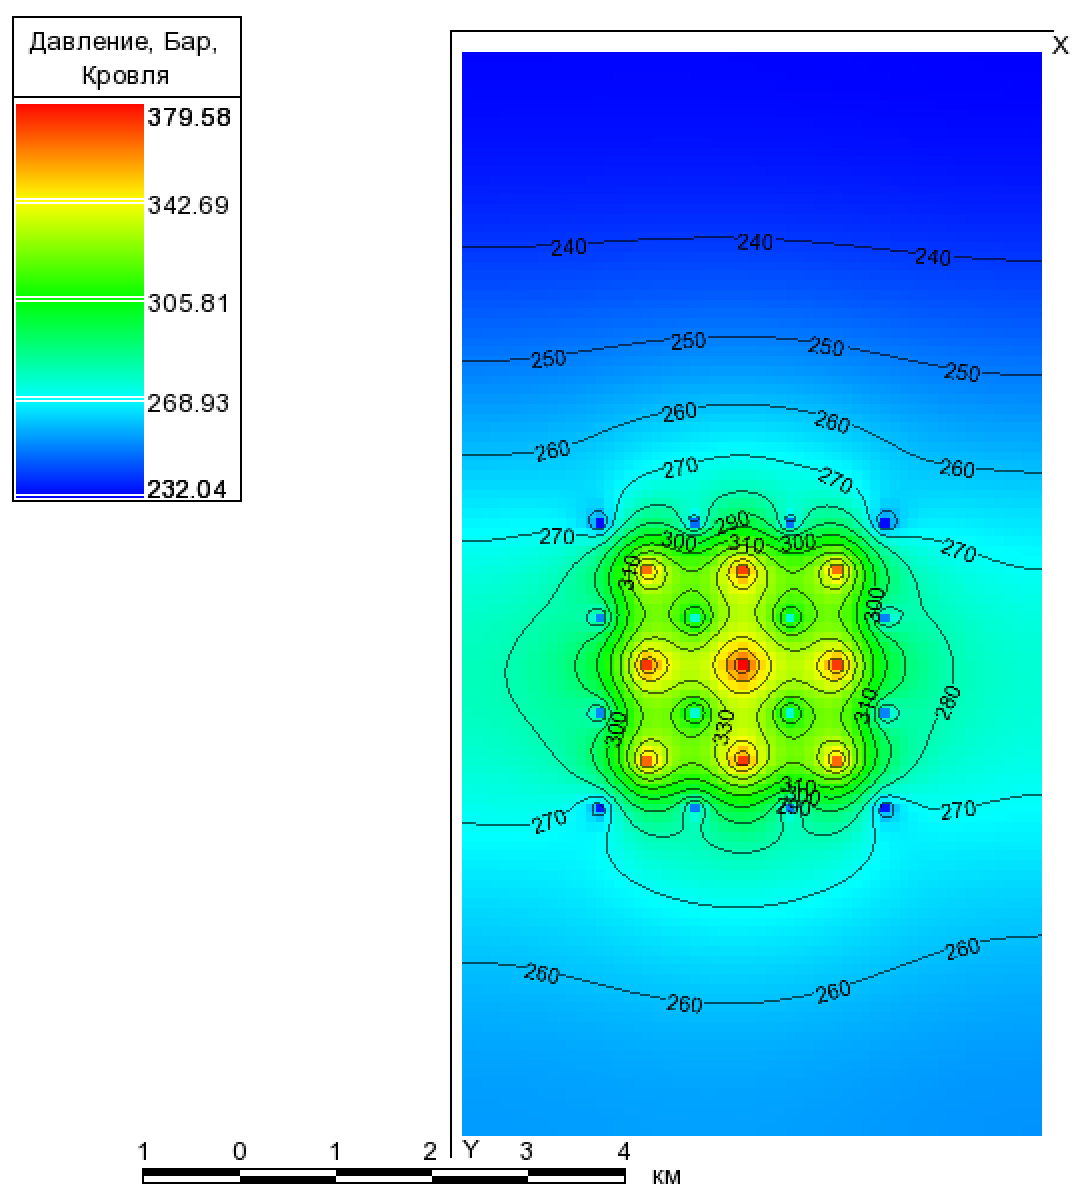
\includegraphics[width=.6\textwidth]{tnav_head_box_pressure_map}
\caption{Распределение давления в последний месяц моделирования -- визуализация tNavigator}
\label{fig:tnav_fwct_box_model}
\end{figure}

\begin{figure}[H]
\center
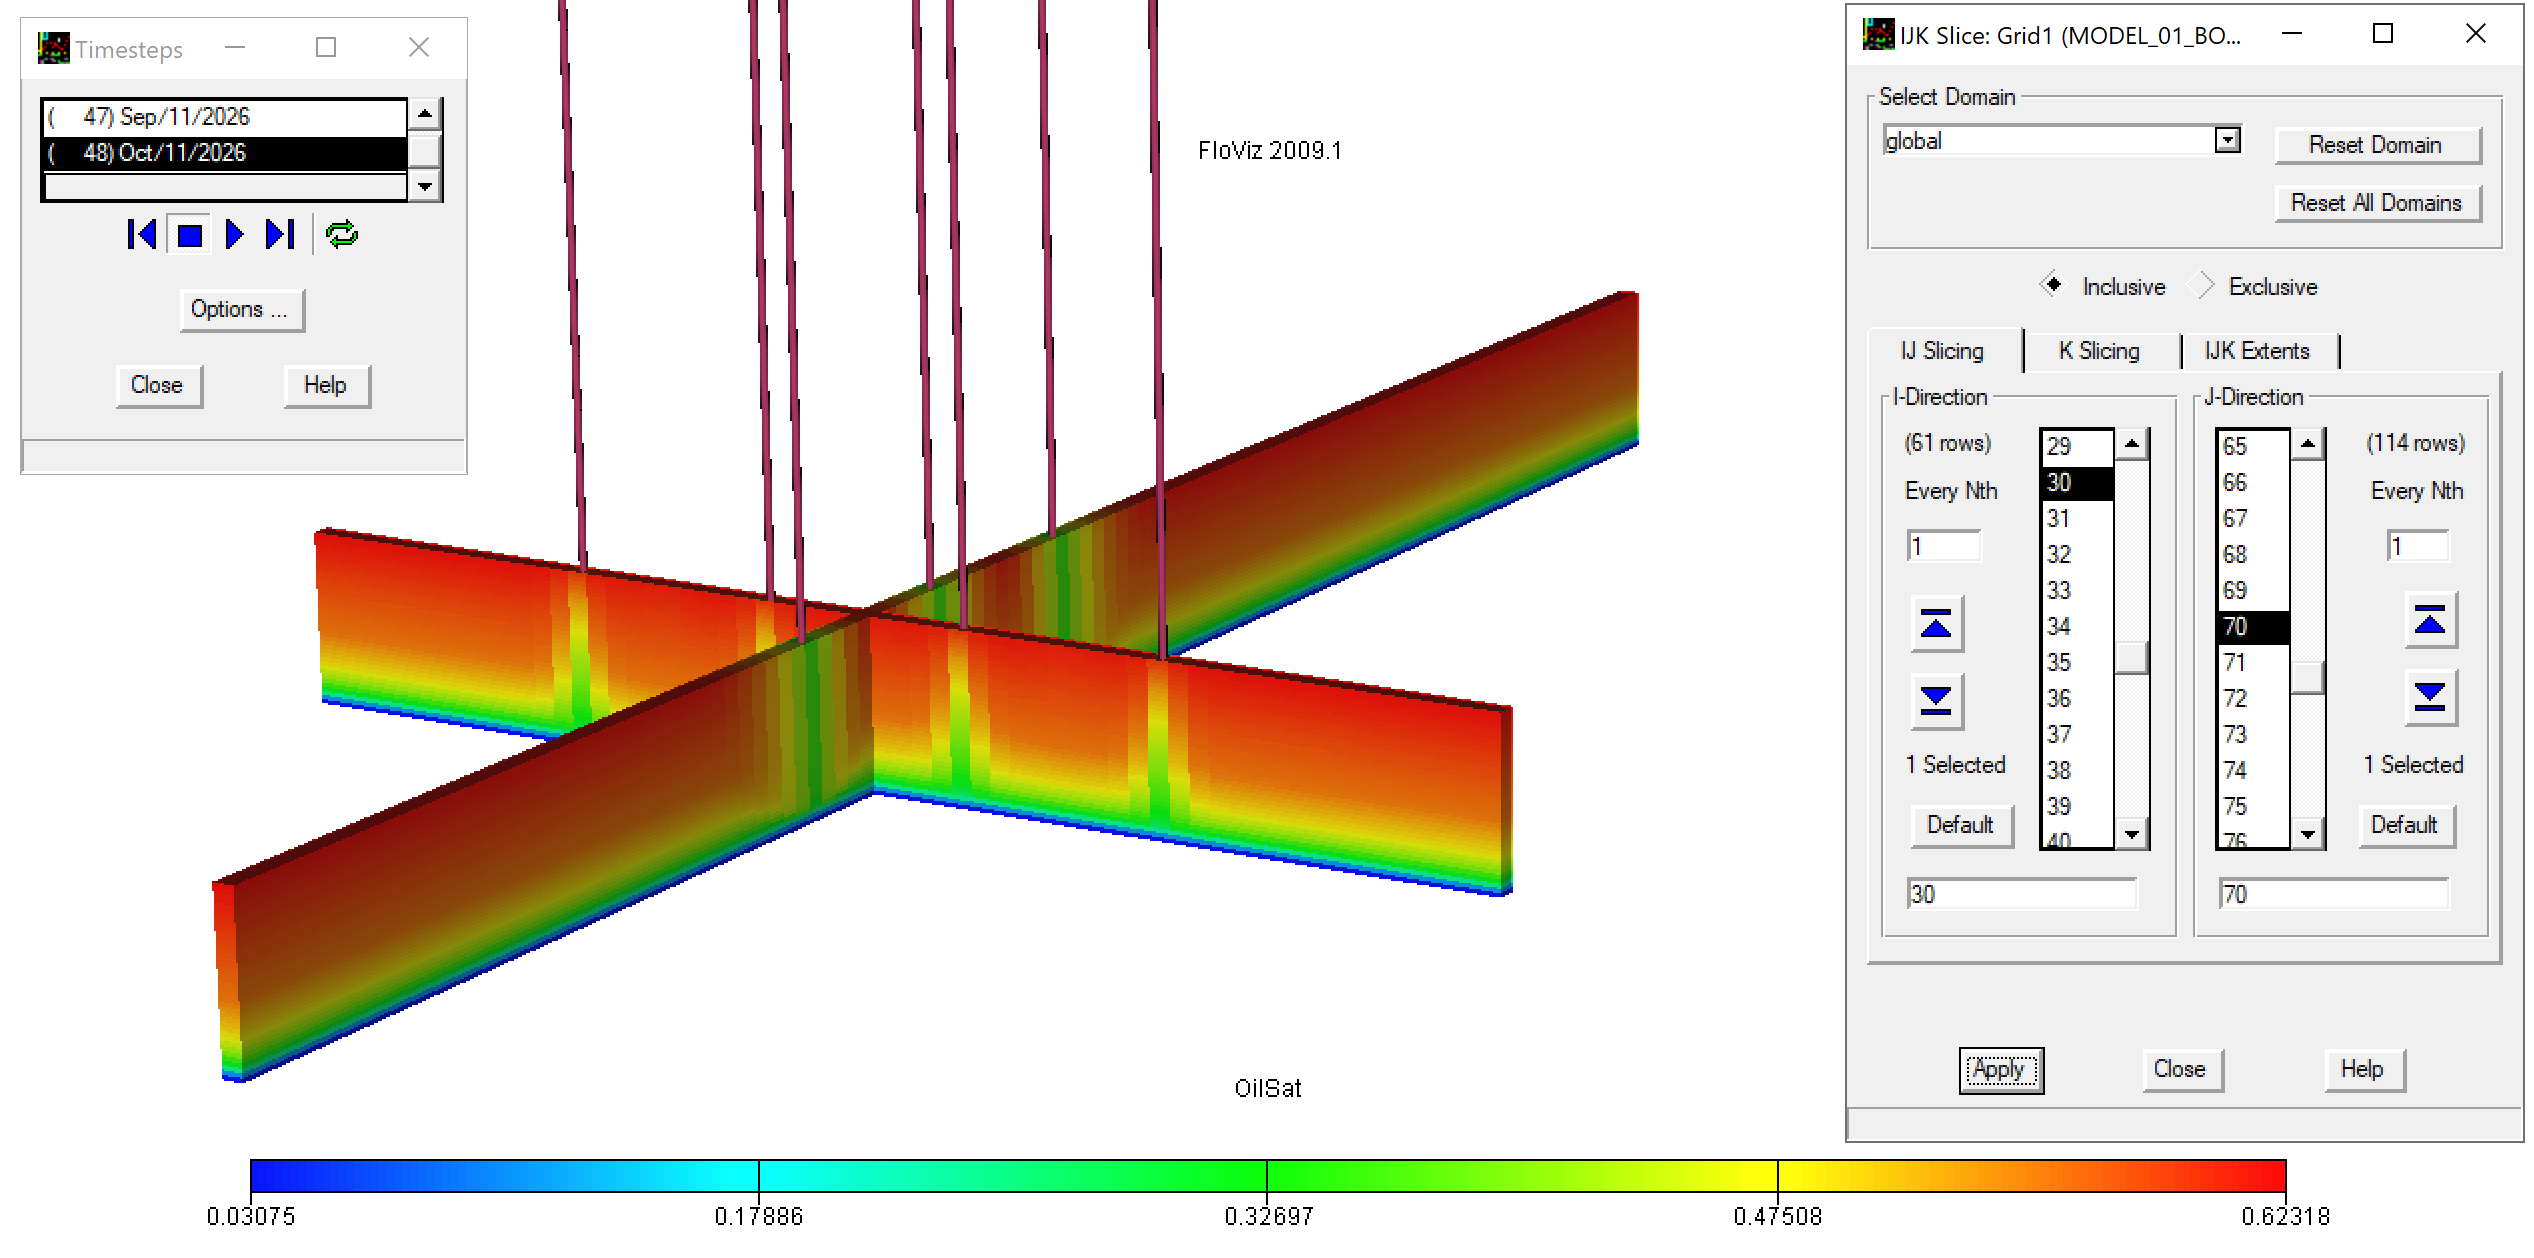
\includegraphics[width=\textwidth]{ecl_oilsat_slices_box_model}
\caption{Нефтенасыщенность в последний месяц моделирования (слайсы вдоль ряда нагнетательных и вдоль ряда добывающих скважин) -- визуализация FloViz}
\label{fig:ecl_oilsat_slices_box_model}
\end{figure}


\begin{figure}[H]
\center
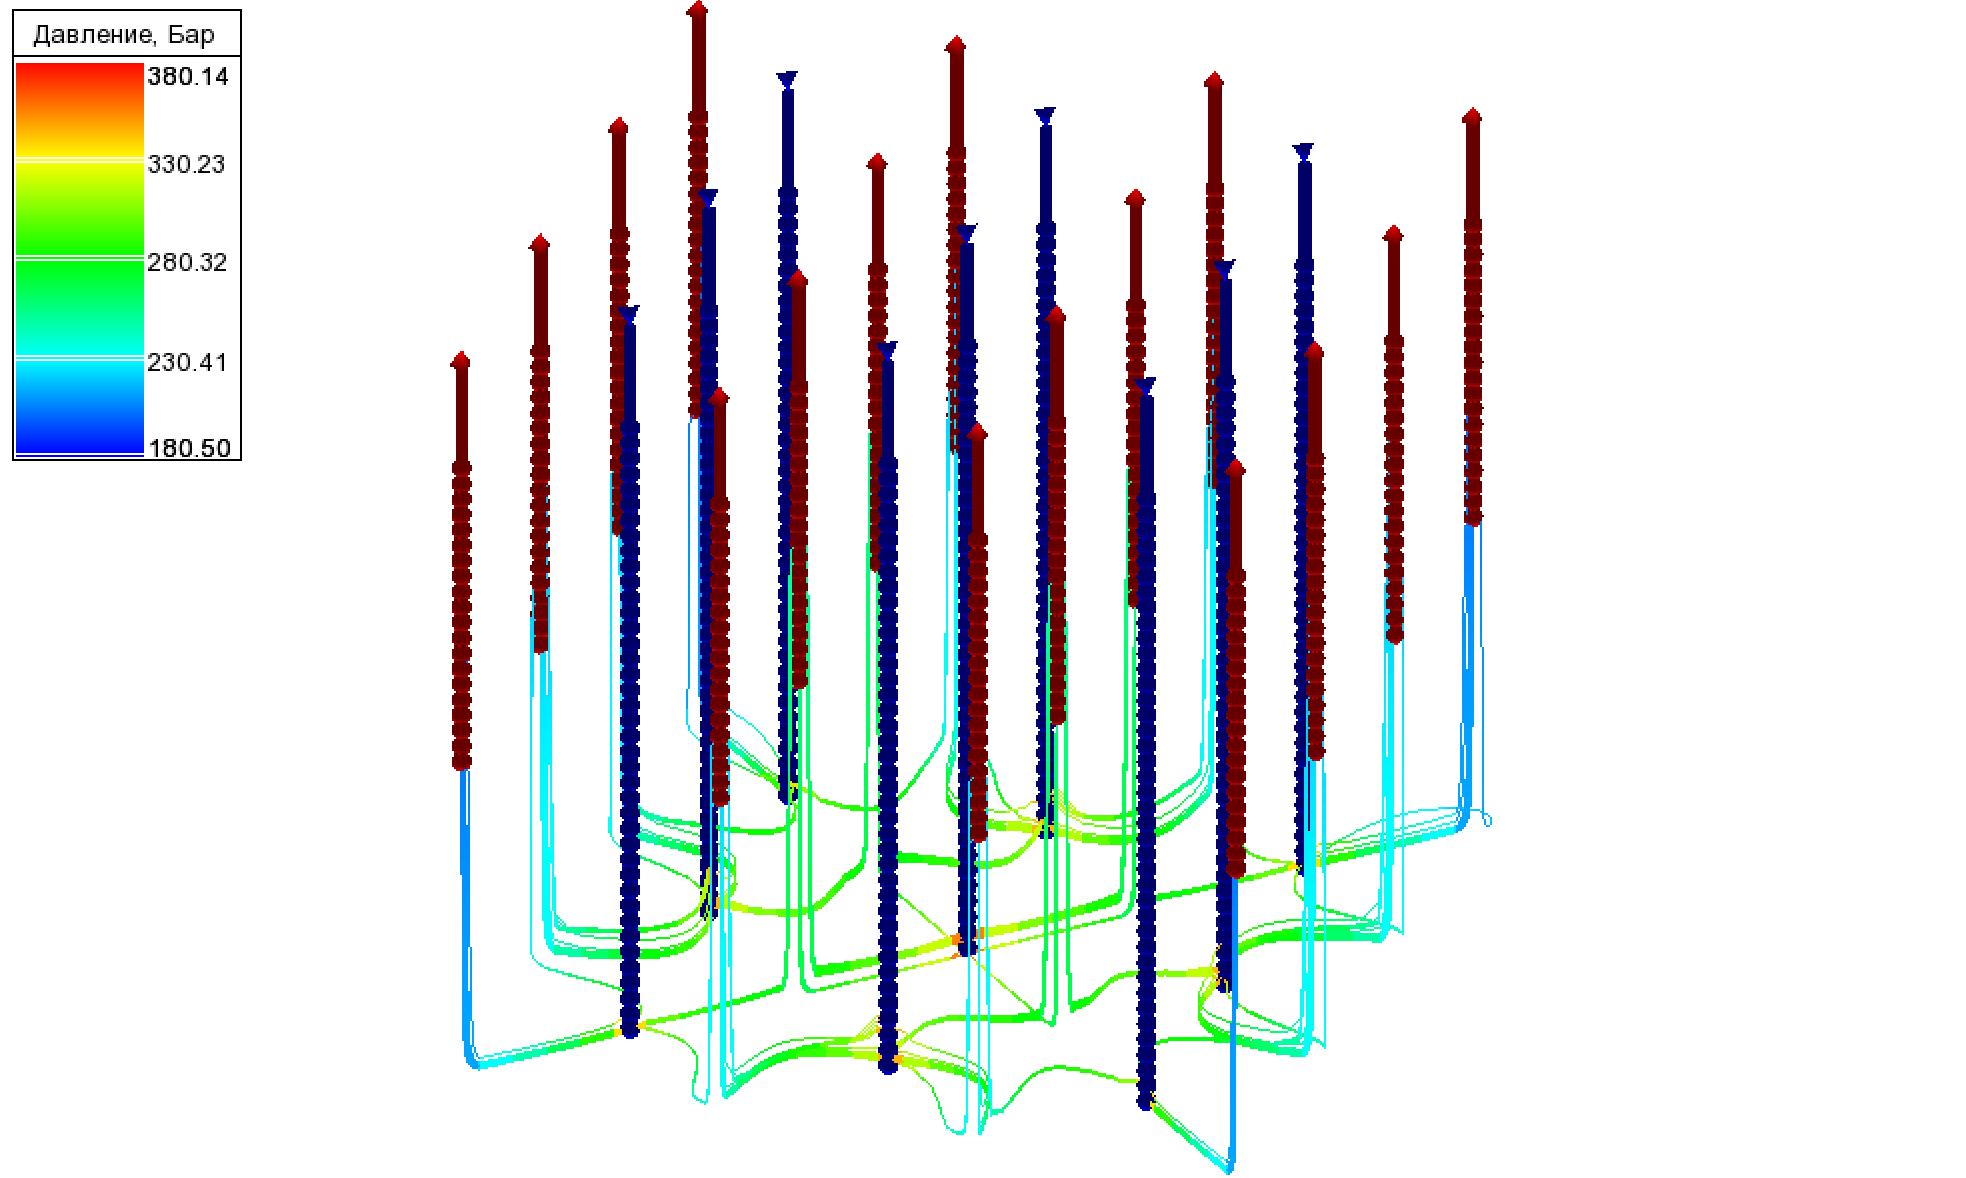
\includegraphics[width=\textwidth]{tnav_flow_lines_start_box_model}
\caption{Линии тока в первые месяцы расчёта -- визуализация tNavigator}
\label{fig:tnav_flow_lines_start_box_model}
\end{figure}

\begin{figure}[H]
\center
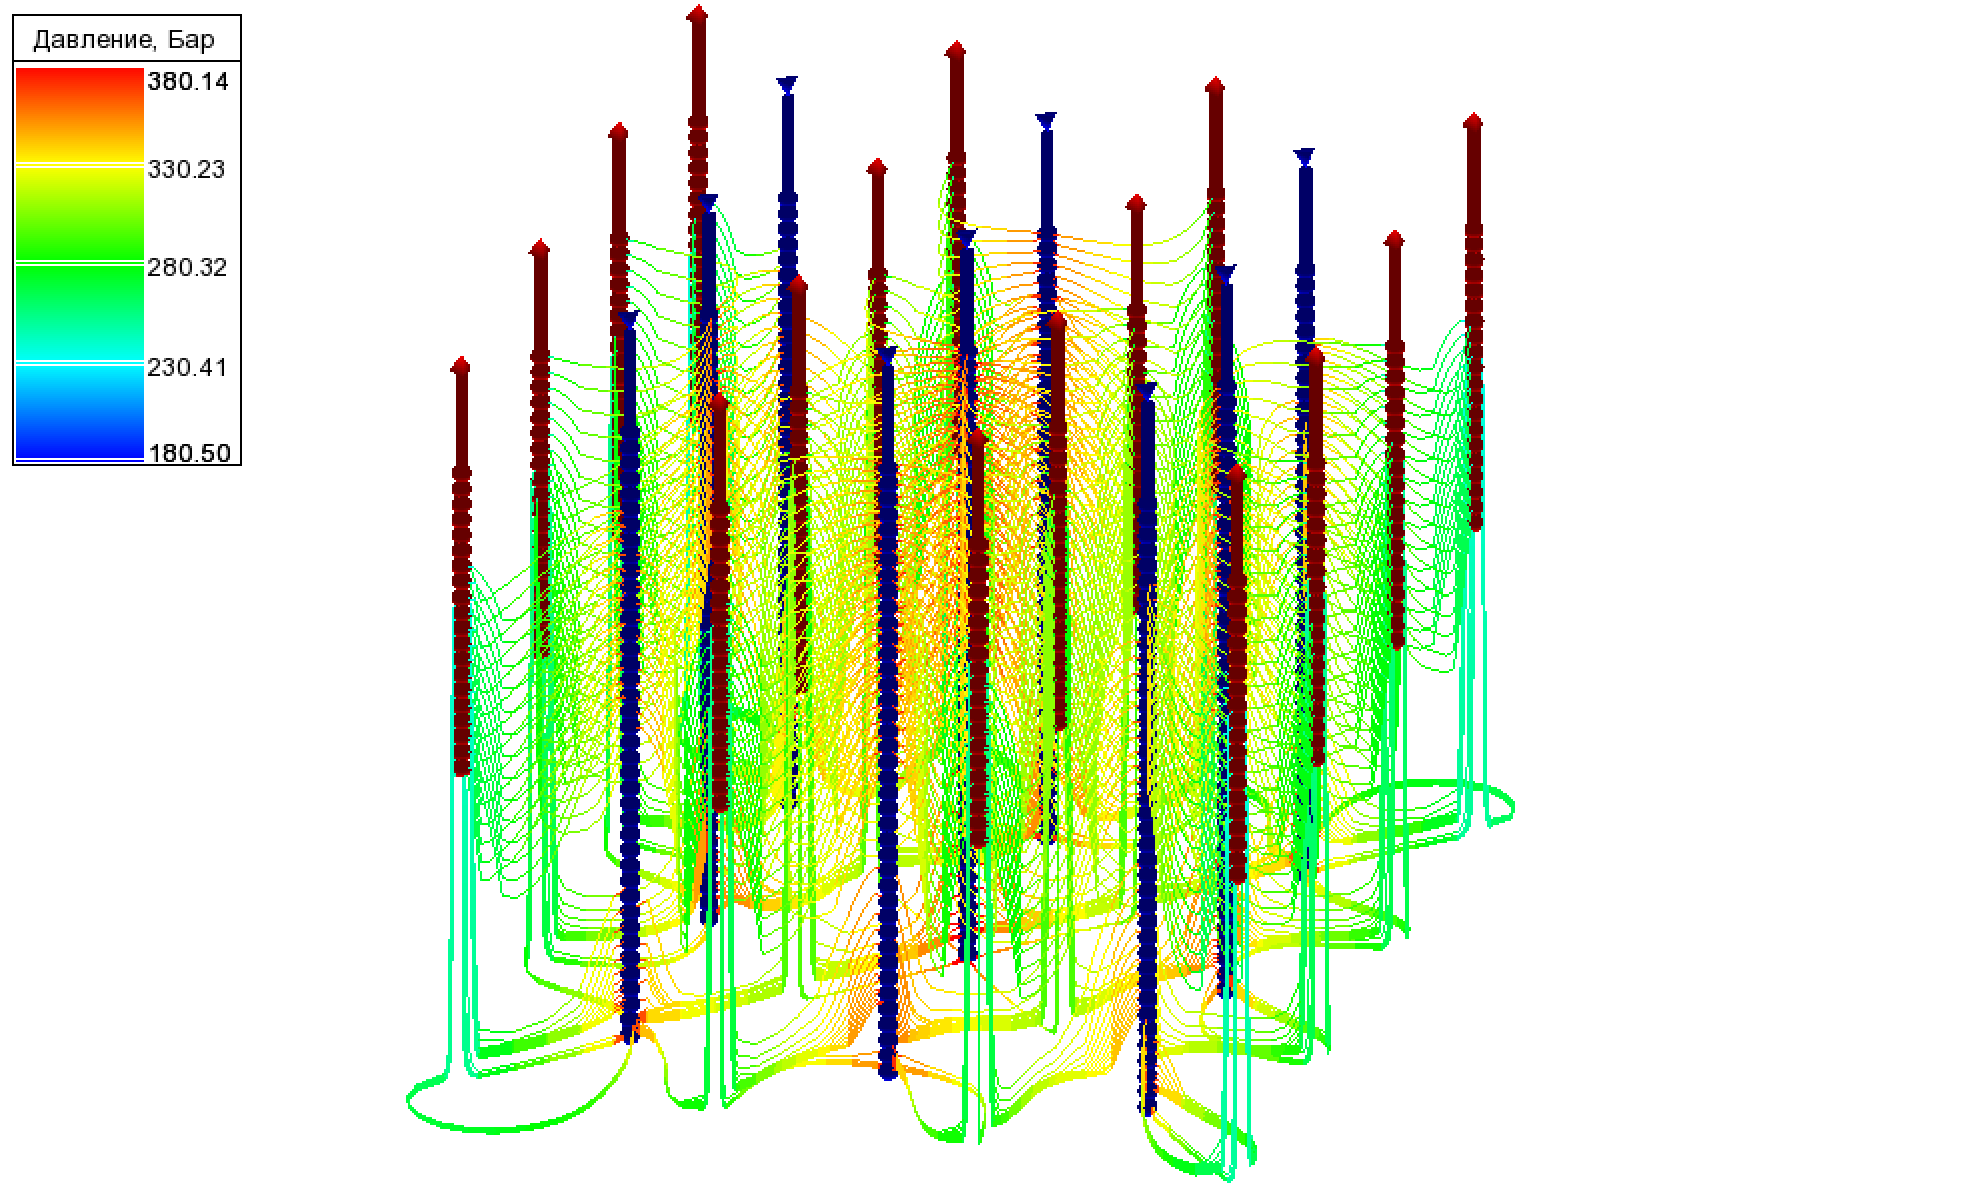
\includegraphics[width=\textwidth]{tnav_flow_lines_end_box_model}
\caption{Линии тока в последний месяц моделирования -- визуализация tNavigator}
\label{fig:tnav_flow_lines_end_box_model}
\end{figure}


\end{document}